\documentclass{article}
\usepackage{amsmath}
\usepackage{amsthm}
\usepackage{color}
\definecolor{orange}{rgb}{0.9,0.4,0} 
\usepackage[colorlinks=true,urlcolor=orange,linkcolor=black]{hyperref}
\usepackage{graphicx}
\usepackage{epigraph}

\newcommand{\libddg}{\texttt{libDDG}\ }

\title{User Guide for \libddg}
\author{Keenan Crane}
\date{October 3, 2011}

\begin{document}

\maketitle

\pagebreak

\tableofcontents

\addtolength{\parskip}{\baselineskip}

\pagebreak
\section{Overview}

\epigraph{\textit{``Premature optimization is the root of all evil.''}}{\textit{Donald Knuth}}

\libddg is a collection of C++ classes designed for use in the Discrete Differential Geometry (DDG) course at the California Institute of Technology and the University of G\"{o}ttingen.  Emphasis is placed on \emph{pedagogy}, \emph{readability}, and \emph{simplicity} -- the goal is to help students quickly prototype and experiment with geometry processing algorithms, and experiment with the design of mesh data structures.  \emph{Note that libDDG is \textbf{not} production-ready code!}  In some cases performance and generality have been compromised for the sake of simplicity and legibility -- students learning differential geometry have enough to worry about without decrypting template metaprograms.

The primary function of \libddg is to build and solve linear algebra problems based on polygonal meshes.  \libddg also includes some facilities for visualization via OpenGL.  The basic idea is that students are given ``bare bones'' data structures and slowly build up additional functionality over the duration of the course.  Certain tasks (such implementing a high-performance, general purpose linear solver) are not the focus of the course -- these components are instead supported by external libraries.

\pagebreak
\section{Acknowledgements}

Thanks to Peter Schr\"{o}der for feedback on library syntax and to Clarisse Weischedel for early beta testing and build support on Linux.

\pagebreak
\section{Getting Started}

To build \libddg you will first need to install and/or build several dependencies: BLAS and SuiteSparse for linear algebra, GLUT and OpenGL for visualization.  \libddg is designed to be used in a POSIX environment (Linux, BSD, Mac OS X, etc.) using the \href{http://en.wikipedia.org/wiki/GNU_toolchain}{GNU toolchain}.  On Windows your best option may be to use \href{http://www.mingw.org/}{MinGW} or \href{http://www.cygwin.com/}{Cygwin}.  (If you are determined to use VisualStudio, see \href{http://matrixprogramming.com/2008/05/umfpack-vc}{Evgenii Rudnyi's article on building SuiteSparse}.)

\subsection{Installing BLAS}

Most platforms include a BLAS implementation by default.  If you do not appear to have BLAS on your system (or do not know where it lives), take a look at

\url{http://www.netlib.org/blas/faq.html}

On Windows/Cygwin, simply (re-)run the Cygwin installer and select all the LAPACK packages in the \textit{Math} category.

\subsection{Installing SuiteSparse}

The exact details of SuiteSparse installation may vary from system to system, but this guide should get you started.  Note that SuiteSparse is installed by default on certain distributions of Linux.  On Windows/Cygwin you can simply select the SuiteSparse packages in the Cygwin installer (and skip the instructions below); however, you may find that you need to manually download the file \href{http://www.cise.ufl.edu/research/sparse/SPQR/SPQR/Include/SuiteSparseQR.hpp}{SuiteSparseQR.hpp} from the \href{http://www.cise.ufl.edu/research/sparse/SPQR/SPQR/}{SuiteSparse home page} and place it in \texttt{C:\\cygdrive\\usr\\include\\suitesparse}.

\begin{enumerate}

\item Download SuiteSparse from

\url{http://www.cise.ufl.edu/research/sparse/SuiteSparse/current/SuiteSparse.tar.gz}

\item Check which version of METIS is currently required by SuiteSparse by checking the \href{http://www.cise.ufl.edu/research/sparse/SuiteSparse/}{SuiteSparse web page}.  As of October 3, 2011 SuiteSparse uses METIS version 4.01, which can be downloaded from

\url{http://glaros.dtc.umn.edu/gkhome/fetch/sw/metis/OLD/metis-4.0.1.tar.gz}

Other versions of METIS can be obtained from the \href{http://glaros.dtc.umn.edu/gkhome/metis/metis/download}{METIS home page}.

\item Unarchive the SuiteSparse distribution.

\item Unarchive the METIS distribution and \emph{put it in the SuiteSparse directory} -- otherwise SuiteSparse will not be able to find METIS.

\item Open \texttt{SuiteSparse/README.txt} -- as mentioned there you will need to edit the file \texttt{SuiteSparse/UFconfig/UFconfig.mk} to specify options for your platform.

\item Type \texttt{make} in the SuiteSparse directory.

\item Type \texttt{sudo make install} in the SuiteSparse directory (you will be prompted for your password).  For some reason SuiteSparse does not always set the correct permissions on header files.  If you are getting ``permission denied'' errors, try typing

\texttt{sudo chmod ugo+r /usr/local/include/*.h /usr/local/include/*.hpp}.

\item Install the METIS library by typing

\texttt{sudo cp metis-4.0/libmetis.a /usr/local/lib}

(or the appropriate subdirectory) in the SuiteSparse root directory.

\end{enumerate}


\subsection{Installing OpenGL/GLUT}

Most platforms include OpenGL and GLUT by default, but if you are on Windows (and not using Cygwin) you will need to install the version of GLUT available here:

\url{http://www.xmission.com/~nate/glut.html}

\subsection{Building libDDG}

Once dependencies are bulit and installed, you must specify their locations by editing the \texttt{Makefile} in the root \texttt{libddg} directory.  Default options for several platforms are available but may need to be modified for your particular environment.  Finally, type \texttt{make} in the root \libddg directory, which builds the executable \texttt{ddg}.  To check if the code was built successfully, run

\texttt{./ddg data/bunny.obj}

which should bring up a window displaying the \href{http://graphics.stanford.edu/software/scanview/models/bunny.html}{Stanford bunny}.

\pagebreak
\section{Basic Routines and Data Structures}

This section gives a high-level introduction to the major classes in \libddg -- for more detailed documentation of individual methods see Section~\ref{sec:libref}.

\subsection{Geometry}

The representation for geometry in \libddg is a bare-bones \emph{halfedge} data structure, which encodes a mesh with polygonal faces.  The idea is that students will extend this data structure over the course of several assignments.  Mesh connectivity is determined by a collection of \emph{halfedges}, which encode the incidence relationships among mesh elements (vertices, edges, and faces):

\vspace{-.3in}
\begin{center}
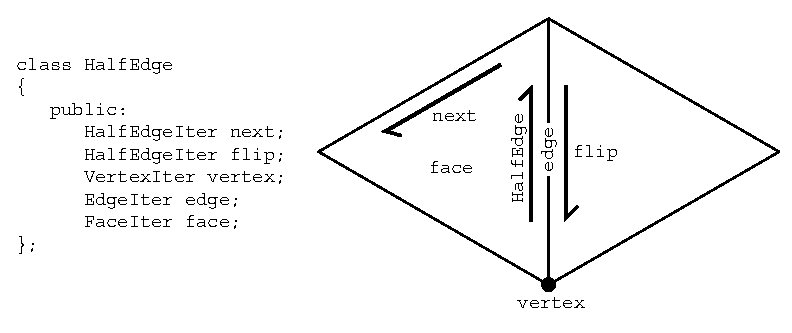
\includegraphics{illustrations/halfedge.pdf}
\end{center}
\vspace{-.3in}

Other mesh elements do not encode connectivity information -- they are used simply as a place to store mesh attributes (normals, colors, etc.).  However, each mesh element stores a reference to one of its halfedges:

\vspace{-.3in}
\begin{center}
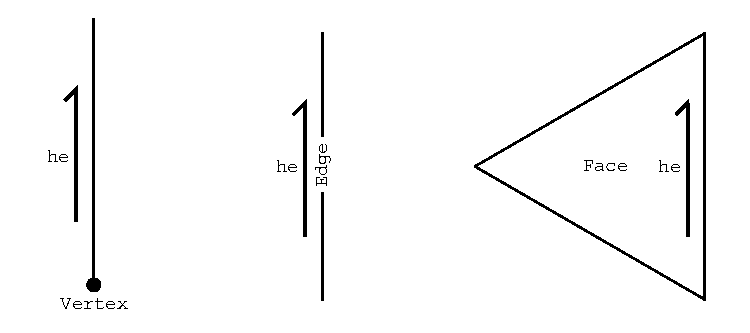
\includegraphics{illustrations/meshelements.pdf}
\end{center}

The primary benefit of the halfedge data structure is that it provides a lot of flexibility for iterating over different mesh regions.  For instance, to iterate over all the vertices of a face \texttt{f} we might write the following loop:

\begin{verbatim}
HalfEdgeIter he = f->he;
do
{
   // do something with he->vertex

   he = he->next;
}
while( he != f->he );
\end{verbatim}

Alternatively, the following loop iterates over all vertices adjacent to a given vertex \texttt{v}:

\begin{verbatim}
HalfEdgeIter he = v->he;
do
{
   // do something with he->flip->vertex

   he = he->flip->next;
}
while( he != v->he );
\end{verbatim}

(Most loops will have this same sort of ``do-while'' structure.)  Note that \emph{by construction} the halfedge data structure can represent only orientable surfaces where every edge is manifold, i.e., every edge is contained in at most two faces.  Non-manifold vertices are possible, however.

\subsubsection{Mesh Attributes}

One challenging question in the design of mesh data structures is: how do you associate data with mesh elements?  Users need to store a variety of different mesh attributes depending on the particular geometry processing problem, but for some reason (possibly related to the available programming paradigms in C++) managing different meshes with different attributes can add considerable complexity to the code.  There are several approaches, but to date it is not clear that one of these approaches is the clear ``winner'' -- \href{http://www.cgal.org/}{CGAL}, \href{http://www.openmesh.org/index.php?id=214}{OpenMesh}, and \href{http://www.cs.sandia.gov/optimization/knupp/Introduction.htm}{Mesquite} demonstrate several possibilities; Seiger and Botsch provide a survey of these data structures and propose an attractive alternative~\cite{Seiger:2011:DIE}.  \libddg remains largely agnostic to this issue, providing only a bare-bones data structure that challenges students to explore these design issues for themselves.

For very simple projects, however, it is usually sufficient to just add mesh attributes directly to element classes.  For instance, to associate a color with each vertex one could modify the \texttt{Vertex} class to look like this:

\begin{verbatim}
class Vertex
{
   public:
      HalfEdgeIter he;

      Vector color; // new attribute
};
\end{verbatim}

\subsubsection{Boundaries}

Surfaces with boundary are handled by treating each boundary loop as an additional face in the mesh.  To determine whether a face \texttt{f} is a boundary face, simply call the routine \texttt{f->isBoundary()}.  For instance, to iterate over all \emph{non}-boundary faces one might write

\begin{verbatim}
for( FaceIter f = faces.begin(); f != faces.end(); f++ )
{
   if( !f->isBoundary() )
   {
      // do some stuff
   }
}
\end{verbatim}

\pagebreak
\subsection{Linear Algebra}

At the most basic level, \libddg provides a wrapper around the SuiteSparse library which can be used to build and solve sparse linear systems.  For instance, to solve the system \(Ax = b\) with

\[ A = \left[\begin{array}{rr} 1 & 3 \\ 2 & 4 \end{array}\right] \]

and

\[ b = \left[\begin{array}{r} 5 \\ 6 \end{array}\right], \]

we can simply write

\begin{verbatim}
SparseMatrix A( 2, 2 );
A(0,0) = 1; A(0,1) = 3;
A(1,0) = 2; A(1,1) = 4;

DenseMatrix b( 2, 1 );
b(0) = 5;
b(1) = 6;

DenseMatrix x( 2, 1 );
solve( A, x, b );
\end{verbatim}

The solution will be stored in the dense vector \texttt{x}.

\subsubsection{Automatic Indexing}

The most meticulous part of geometry processing is often establishing a correspondence between mesh elements and variables in a linear system.  The usual idea is that each element is given a unique integer ID which is used as a row or column index in a matrix.  In many cases, however, there is no good reason for the programmer to think about a linear system in terms of matrices, indices, and so forth.  In these situations, \libddg provides an abstraction that automatically handles variable indexing and indeed the entire process of solving a linear system.  This abstraction is especially useful for debugging and rapid prototyping (though it should be noted that better performance can often be achieved by building matrices ``by hand.'')
 
For example, suppose one wants to solve the linear system

\[
   \begin{array}{rcl}
        3(x+y/2) + z &=& 4 \\
                 z-8 &=& y+x/9 \\
   (x+y)/5 + (y+z)/6 &=& 7 \\
   \end{array}
\]

for the values \(x\), \(y\), and \(z\).  In \libddg this system can be solved by simply writing

\begin{verbatim}
LinearSystem sys;
Variable x, y, z;

sys.push_back(     3*(x+y/2) + z == 4     );
sys.push_back(               z-8 == y+x/9 );
sys.push_back( (x+y)/5 + (y+z)/6 == 7     );

sys.solve();
\end{verbatim}

There are a few things to note here.  First, we did not need to put the equations into some kind of special form (e.g., we did not have to move all terms to the left-hand side or expand the expression in terms of primary variables).  This kind of flexibility makes it easy to verify \emph{visually} that we typed in the right set of equations.  Second, note that the method \texttt{LinearSystem::solve()} automatically copies the solution of the system back into our variables \texttt{x}, \texttt{y}, and \texttt{z}.  For instance, if we now wanted to display the solution we could simply write

\begin{verbatim}
cout << "x: " << *x << endl;
cout << "y: " << *y << endl;
cout << "z: " << *z << endl;
\end{verbatim}

Here the dereference operator (\texttt{*}) is used to access the numerical value stored in each variable (whereas variables are typically treated as purely symbolic objects).

\subsubsection{Fixed Variables}

In many cases it is useful to be able to \emph{fix} certain variables (i.e., hold their values constant) while solving a linear system -- for instance, one might want to prescribe boundary conditions in a finite element problem.  In \libddg, variables can be fixed by setting the flag \texttt{Variable::fixed}.  For instance, consider the system

\[
   \begin{array}{rcl}
   x + y &=& a \\
   x - y &=& b
   \end{array}
\]

which can be encoded via

\begin{verbatim}
LinearSystem sys;
Variable x, y, a, b;

sys.push_back( x + y == a );
sys.push_back( x - y == b );
\end{verbatim}

Initially, all the variables (\(x\), \(y\), \(a\), and \(b\)) are degrees of freedom in our system.  To fix the values on the right hand, we simply write

\begin{verbatim}
a.fixed = true;
b.fixed = true;
\end{verbatim}

Now when we call \(sys.solve()\), the variables \texttt{a} and \texttt{b} will automatically be interpreted as constants.  For instance, to solve a sequence of systems with different right-hand sides we could write

\begin{verbatim}
*a = 1;
*b = 2;
sys.solve();

*a = 3;
*b = 4;
sys.solve();
\end{verbatim}

Moreover, we can dynamically change the set of fixed variables.  For instance, to keep \texttt{x} and \texttt{y} fixed while solving for \texttt{a} and \texttt{b}, we would write something like

\pagebreak

\begin{verbatim}

a.fixed = false;
b.fixed = false;

x.fixed = true;
y.fixed = true;

*x = 1.23;
*y = 4.56;

sys.solve();
\end{verbatim}

\pagebreak
\subsection{Visualization}

\begin{center}
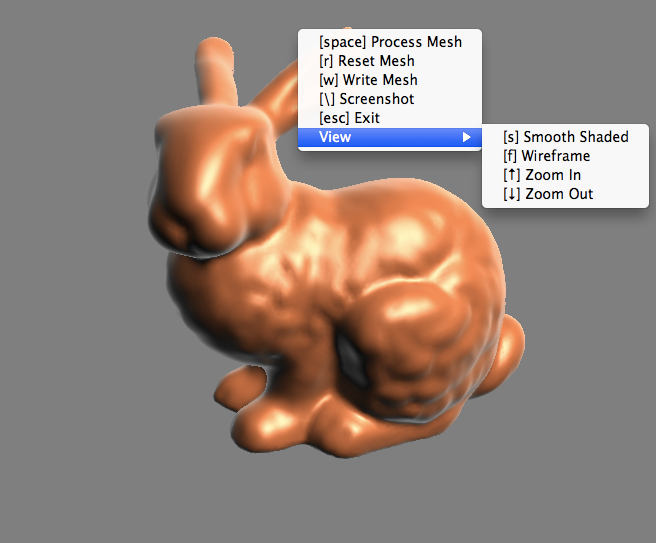
\includegraphics[width=.7\columnwidth]{illustrations/viewer.png}
\end{center}

The \texttt{Viewer} class provides basic facilities for inspecting and interacting with a mesh.  Additional functionality can be added using OpenGL, GLUT, and GLSL (see \href{http://nehe.gamedev.net/}{NeHe} for a nice collection of OpenGL/GLUT tutorials).  Setting up a viewer for a mesh can be done in just three lines:

\begin{verbatim}
Viewer viewer;
viewer.mesh.read( meshFilename );
viewer.init();
\end{verbatim}

which should bring up a viewer window similar to the one pictured above.  Right-clicking on this window brings up a list of commands and their keyboard equivalents.

\pagebreak
\section{Library Reference}
\label{sec:libref}

\addtolength{\parskip}{-\baselineskip}

\subsection{DenseMatrix}

DenseMatrix represents an m by n (real or complex) matrix where every entry -- including zero-valued entries -- is stored explicitly.  This class is most commonly used to represent dense vectors in sparse linear systems (i.e., the right hand side and the solution vector). 

 A real or complex matrix is allocated via 

 \begin{verbatim}
     DenseMatrix A( m, n );
     DenseMatrix A( m, n, Complex );
 \end{verbatim}
\vspace{-\baselineskip} Matrix elements are then accessed using parenthesis, e.g., 

 \begin{verbatim}
     A(i,j) = 1;
     A(i,j) += 2;
     a = A(i,j);
 \end{verbatim}
\vspace{-\baselineskip} etc. 

 DenseMatrix is interoperable with the SuiteSparse numerical linear algebra library.  In particular, dereferencing a DenseMatrix returns a cholmod\_dense* which can be used by routines in SuiteSparse.  For basic operations, however, \begin{verbatim}
  you should not need to access this pointer explicitly -- see the solve()
 method in SparseMatrix.h.\end{verbatim}
\vspace{-\baselineskip} 

\subsubsection{Class Reference}

\rule{5in}{1pt}
\begin{verbatim}
DenseMatrix( int m = 0, int n = 0, int xtype = Real );
\end{verbatim}
\textbf{Purpose:}
initialize an mxn matrix of doubles
xtype is either DDG::Real or DDG::Complex

\hspace{-.21in}\rule{5in}{1pt}
\begin{verbatim}
DenseMatrix( const DenseMatrix& A );
\end{verbatim}
\textbf{Purpose:}
copy constructor

\hspace{-.21in}\rule{5in}{1pt}
\begin{verbatim}
const DenseMatrix& operator=( const DenseMatrix& A );
\end{verbatim}
\textbf{Purpose:}
copies A

\hspace{-.21in}\rule{5in}{1pt}
\begin{verbatim}
~DenseMatrix( void );
\end{verbatim}
\textbf{Purpose:}
destructor

\hspace{-.21in}\rule{5in}{1pt}
\begin{verbatim}
int nRows( void ) const;
\end{verbatim}
\textbf{Purpose:}
returns the number of rows

\hspace{-.21in}\rule{5in}{1pt}
\begin{verbatim}
int nColumns( void ) const;
\end{verbatim}
\textbf{Purpose:}
returns the number of columns

\hspace{-.21in}\rule{5in}{1pt}
\begin{verbatim}
int length( void ) const;
\end{verbatim}
\textbf{Purpose:}
returns the size of the largest dimension

\hspace{-.21in}\rule{5in}{1pt}
\begin{verbatim}
void zero( double rVal = 0., double iVal = 0. );
\end{verbatim}
\textbf{Purpose:}
sets all elements to rVal+iVal*i

\hspace{-.21in}\rule{5in}{1pt}
\begin{verbatim}
double norm( void );
\end{verbatim}
\textbf{Purpose:}
returns the maximum magnitude of any entry

\hspace{-.21in}\rule{5in}{1pt}
\begin{verbatim}
double& operator()( int row, int col );
double  operator()( int row, int col ) const;
double& r( int row, int col );
double  r( int row, int col ) const;
\end{verbatim}
\textbf{Purpose:}
access real part of element (row,col)
note: uses 0-based indexing

\hspace{-.21in}\rule{5in}{1pt}
\begin{verbatim}
double& i( int row, int col );
double  i( int row, int col ) const;
\end{verbatim}
\textbf{Purpose:}
access imaginary part of element (row,col)
note: uses 0-based indexing

\hspace{-.21in}\rule{5in}{1pt}
\begin{verbatim}
double& operator()( int index );
double  operator()( int index ) const;
\end{verbatim}
\textbf{Purpose:}
access real part of element ind of a vector
note: uses 0-based indexing

\hspace{-.21in}\rule{5in}{1pt}
\begin{verbatim}
double& r( int index );
double  r( int index ) const;
\end{verbatim}
\textbf{Purpose:}
access real part of element ind of a vector
note: uses 0-based indexing

\hspace{-.21in}\rule{5in}{1pt}
\begin{verbatim}
double& i( int index );
double  i( int index ) const;
\end{verbatim}
\textbf{Purpose:}
access imaginary part of element ind of a vector
note: uses 0-based indexing

\hspace{-.21in}\rule{5in}{1pt}
\begin{verbatim}
DenseMatrix transpose( void ) const;
\end{verbatim}
\textbf{Purpose:}
returns the transpose of this matrix

\hspace{-.21in}\rule{5in}{1pt}
\begin{verbatim}
DenseMatrix operator*( const DenseMatrix& B ) const;
\end{verbatim}
\textbf{Purpose:}
returns product of this matrix with B

\hspace{-.21in}\rule{5in}{1pt}
\begin{verbatim}
void operator*=( double c );
\end{verbatim}
\textbf{Purpose:}
multiplies this matrix by the scalar c

\hspace{-.21in}\rule{5in}{1pt}
\begin{verbatim}
void operator/=( double c );
\end{verbatim}
\textbf{Purpose:}
divides this matrix by the scalar c

\hspace{-.21in}\rule{5in}{1pt}
\begin{verbatim}
DenseMatrix operator+( const DenseMatrix& B ) const;
\end{verbatim}
\textbf{Purpose:}
returns sum of this matrix with B

\hspace{-.21in}\rule{5in}{1pt}
\begin{verbatim}
DenseMatrix operator-( const DenseMatrix& B ) const;
\end{verbatim}
\textbf{Purpose:}
returns difference of this matrix with B

\hspace{-.21in}\rule{5in}{1pt}
\begin{verbatim}
cholmod_dense* operator*( void ) const;
\end{verbatim}
\textbf{Purpose:}
returns pointer to underlying cholmod\_dense data structure

\hspace{-.21in}\rule{5in}{1pt}
\begin{verbatim}
const DenseMatrix& operator=( cholmod_dense* A );
\end{verbatim}
\textbf{Purpose:}
gets pointer to A; will deallocate A upon destruction

\pagebreak
\subsection{Edge}

 

 Edge stores attributes associated with a mesh edge.  The iterator he points to one of its two associated halfedges.  (See the documentation for a more in-depth discussion of the halfedge data structure.) 



\subsubsection{Class Reference}

\rule{5in}{1pt}
\begin{verbatim}
HalfEdgeIter he;
\end{verbatim}
\textbf{Purpose:}
points to one of the two halfedges associated with this edge
\pagebreak\subsection{Face}

 

 Face stores attributes associated with a mesh edge.  The iterator he points to one of its associated halfedges.  (See the documentation for a more in-depth discussion of the halfedge data structure.) 



\subsubsection{Class Reference}

\rule{5in}{1pt}
\begin{verbatim}
HalfEdgeIter he;
\end{verbatim}
\textbf{Purpose:}
points to one of the halfedges associated with this face

\hspace{-.21in}\rule{5in}{1pt}
\begin{verbatim}
bool isBoundary( void ) const;
\end{verbatim}
\textbf{Purpose:}
returns true if this face corresponds to a
boundary loop; false otherwise

\hspace{-.21in}\rule{5in}{1pt}
\begin{verbatim}
Vector normal( void ) const;
\end{verbatim}
\textbf{Purpose:}
returns the unit normal associated with this face; normal
orientation is determined by the circulation order of halfedges
\pagebreak\subsection{HalfEdge}

 

 HalfEdge is used to define mesh connectivity.  (See the documentation for a more in-depth discussion of the halfedge data structure.) 



\subsubsection{Class Reference}

\rule{5in}{1pt}
\begin{verbatim}
HalfEdgeIter next;
\end{verbatim}
\textbf{Purpose:}
points to the next halfedge around the current face

\hspace{-.21in}\rule{5in}{1pt}
\begin{verbatim}
HalfEdgeIter flip;
\end{verbatim}
\textbf{Purpose:}
points to the other halfedge associated with this edge

\hspace{-.21in}\rule{5in}{1pt}
\begin{verbatim}
VertexIter vertex;
\end{verbatim}
\textbf{Purpose:}
points to the vertex at the ``tail'' of this halfedge

\hspace{-.21in}\rule{5in}{1pt}
\begin{verbatim}
EdgeIter edge;
\end{verbatim}
\textbf{Purpose:}
points to the edge associated with this halfedge

\hspace{-.21in}\rule{5in}{1pt}
\begin{verbatim}
FaceIter face;
\end{verbatim}
\textbf{Purpose:}
points to the face containing this halfedge

\hspace{-.21in}\rule{5in}{1pt}
\begin{verbatim}
bool onBoundary;
\end{verbatim}
\textbf{Purpose:}
true if this halfedge is contained in a boundary
loop; false otherwise

\hspace{-.21in}\rule{5in}{1pt}
\begin{verbatim}
Vector texcoord;
\end{verbatim}
\textbf{Purpose:}
texture coordinates associated with the triangle corner at the
``tail'' of this halfedge
\pagebreak\subsection{Image}

 Image represents a color bitmap image.  A simple example might look like 

 \begin{verbatim}
     Image im;
     im.read( "input.tga" );
     // modify image data via im(x,y) = ...;
     im.write( "output.tga" );
 \end{verbatim}
\vspace{-\baselineskip}

\subsubsection{Class Reference}

\rule{5in}{1pt}
\begin{verbatim}
Image( int width = 0, int height = 0 );
\end{verbatim}
\textbf{Purpose:}
constructs image with specified width and height

\hspace{-.21in}\rule{5in}{1pt}
\begin{verbatim}
float& operator()( int x, int y );
const float& operator()( int x, int y ) const;
\end{verbatim}
\textbf{Purpose:}
accesses pixel (x,y)

\hspace{-.21in}\rule{5in}{1pt}
\begin{verbatim}
float sample( float x, float y ) const;
\end{verbatim}
\textbf{Purpose:}
samples image at (x,y) using bilinear filtering

\hspace{-.21in}\rule{5in}{1pt}
\begin{verbatim}
int  width( void ) const;
int height( void ) const;
\end{verbatim}
\textbf{Purpose:}
returns image dimensions

\hspace{-.21in}\rule{5in}{1pt}
\begin{verbatim}
void read( const char* filename );
\end{verbatim}
\textbf{Purpose:}
loads an image file in Truevision TGA format
(must be RGB image with 24 or 32 bits per pixel)

\hspace{-.21in}\rule{5in}{1pt}
\begin{verbatim}
void write( const char* filename ) const;
\end{verbatim}
\textbf{Purpose:}
writes an image file in Truevision TGA format
(RGB image with 24 bits per pixel)
\pagebreak\subsection{LinearContext}

 

 LinearContext is the global solver context needed to interface with the SuiteSparse library.  It is essentially a wrapper around cholmod\_common.  A single static instance of LinearContext is declared in LinearContext.cpp and is shared by all instances of DenseMatrix, SparseMatrix, and LinearSystem. In other words, you shouldn't have to instantiate LinearContext yourself unless you're doing something really fancy! 



\subsubsection{Class Reference}

\rule{5in}{1pt}
\begin{verbatim}
LinearContext( void );
\end{verbatim}
\textbf{Purpose:}
constructor

\hspace{-.21in}\rule{5in}{1pt}
\begin{verbatim}
~LinearContext( void );
\end{verbatim}
\textbf{Purpose:}
destructor

\hspace{-.21in}\rule{5in}{1pt}
\begin{verbatim}
operator cholmod_common*( void );
\end{verbatim}
\textbf{Purpose:}
allows LinearContext to be treated as a cholmod\_common*

\pagebreak\subsection{LinearEquation}

 

 LinearEquation represents an equation with an arbitrary linear polynomial on both the left- and right-hand side.  It is primarily used while building a LinearSystem.  For convenience, operator== is overloaded so that the user can construct a LinearEquation by writing something that looks much like the usual mathematical syntax for a linear equation.  For example, 

 \begin{verbatim}
     LinearEquation eqn = ( x + 2*y == 3*z );
 \end{verbatim}
\vspace{-\baselineskip} builds the linear equation x + 2y = 3z. 



\subsubsection{Class Reference}

\rule{5in}{1pt}
\begin{verbatim}
LinearPolynomial lhs;
\end{verbatim}
\textbf{Purpose:}
left-hand side

\hspace{-.21in}\rule{5in}{1pt}
\begin{verbatim}
LinearPolynomial rhs;
\end{verbatim}
\textbf{Purpose:}
right-hand side
\pagebreak\subsection{LinearPolynomial}

 

 LinearPolynomial represents an affine function of the form 

 \[ f(x_1,x_2,...,x_n) = c_1 x_1 + c_2 x_2 + ... + c_n x_n + d \]

 where the \(x_i\) are real-valued variables with real coefficients \(c_i\), and \(d\) is a real constant.  The variables and their coefficients are represented using instances of the Variable class.  LinearPolynomial implements all the usual algebraic operations on affine functions, as well as type conversions from more elementary types (scalars, single variables, etc.). 

 Importantly, variables used in a LinearPolynomial should \textbf{not} be deallocated while the polynomial is still in use -- LinearPolynomial stores only a reference to these variables so that the solution to a linear system can be automatically copied back into the variables. 



\subsubsection{Class Reference}

\rule{5in}{1pt}
\begin{verbatim}
LinearPolynomial( void );
\end{verbatim}
\textbf{Purpose:}
constructs the zero function

\hspace{-.21in}\rule{5in}{1pt}
\begin{verbatim}
LinearPolynomial( double c );
\end{verbatim}
\textbf{Purpose:}
constructs the constant function with value c

\hspace{-.21in}\rule{5in}{1pt}
\begin{verbatim}
LinearPolynomial( Variable& v );
\end{verbatim}
\textbf{Purpose:}
constructs a function with a single variable v

\hspace{-.21in}\rule{5in}{1pt}
\begin{verbatim}
const LinearPolynomial& operator=( double c );
\end{verbatim}
\textbf{Purpose:}
assigns the constant function with value c

\hspace{-.21in}\rule{5in}{1pt}
\begin{verbatim}
const LinearPolynomial& operator=( Variable& v );
\end{verbatim}
\textbf{Purpose:}
assigns a function with a single variable v

\hspace{-.21in}\rule{5in}{1pt}
\begin{verbatim}
void operator+=( double c );
void operator-=( double c );
void operator*=( double c );
void operator/=( double c );
\end{verbatim}
\textbf{Purpose:}
adds, subtract, multiplies, or divides by a constant

\hspace{-.21in}\rule{5in}{1pt}
\begin{verbatim}
void operator+=( Variable& v );
void operator-=( Variable& v );
\end{verbatim}
\textbf{Purpose:}
increments or decrements by a single variable v

\hspace{-.21in}\rule{5in}{1pt}
\begin{verbatim}
void operator+=( const LinearPolynomial& p );
void operator-=( const LinearPolynomial& p );
\end{verbatim}
\textbf{Purpose:}
increments or decrements by an affine function

\hspace{-.21in}\rule{5in}{1pt}
\begin{verbatim}
LinearPolynomial operator-( void ) const;
\end{verbatim}
\textbf{Purpose:}
returns the additive inverse (i.e., negation)

\hspace{-.21in}\rule{5in}{1pt}
\begin{verbatim}
double evaluate( void ) const;
\end{verbatim}
\textbf{Purpose:}
evaluates the function using the current values of its variables

\hspace{-.21in}\rule{5in}{1pt}
\begin{verbatim}
std::map<Variable*,double> linearTerms;
\end{verbatim}
\textbf{Purpose:}
list of linear terms

\hspace{-.21in}\rule{5in}{1pt}
\begin{verbatim}
double constantTerm;
\end{verbatim}
\textbf{Purpose:}
constant term
\pagebreak\subsection{LinearSystem}

 

 LinearSystem represents a system of linear equations expressed in terms of instances of the Variable class.  The main idea is to make it easy to construct and solve linear systems without explicitly think about variable indices, matrix layout, etc.  (This kind of abstraction is particularly useful for debugging and rapid prototyping.)  See the documentation for examples of building linear and solving systems. 

 Importantly, any variable used by a LinearSystem should not be deallocated while the system is still in use, because the method LinearSystem::solve() automatically copies the solution back into the variables used to define the equations.  (In the future variables may become reference-counted in order to avoid this issue.) 

 Note that LinearSystem::solve() uses a general-purpose linear solver (namely the sparse QR factorization found in SuiteSparse) that is quite fast but may not always be your best option.  To improve performance you may want to build the system explicitly using an instance of SparseMatrix and call a more specialized solver.  (In the future there may be options for specifying that a LinearSystem is, e.g., symmetric and positive-definite.) 



\subsubsection{Class Reference}

\rule{5in}{1pt}
\begin{verbatim}
void clear( void );
\end{verbatim}
\textbf{Purpose:}
removes all equations from the system

\hspace{-.21in}\rule{5in}{1pt}
\begin{verbatim}
void push_back( const LinearEquation& e );
\end{verbatim}
\textbf{Purpose:}
appends the equation e to the sytem

\hspace{-.21in}\rule{5in}{1pt}
\begin{verbatim}
void solve( void );
\end{verbatim}
\textbf{Purpose:}
solves the system and automatically stores the result in the variables
for an overdetermined system, computes a least-squares solution

\hspace{-.21in}\rule{5in}{1pt}
\begin{verbatim}
std::vector<LinearEquation> equations;
\end{verbatim}
\textbf{Purpose:}
the collection of equations defining the system

\pagebreak\subsection{Mesh}

 

 Mesh represents a polygonal surface mesh using the halfedge data structure. It is essentially a large collection of disjoint vertices, edges, and faces that are ``glued together'' by halfedges which encode connectivity (see the documentation for an illustration).  By construction, the halfedge data structure cannot represent nonorientable surfaces or meshes with nonmanifold edges. 

 Mesh elements are referenced using iterators -- common usage of these iterators is to either traverse an entire vector of mesh elements: 

 \begin{verbatim}
     // visit all vertices
     for( VertexIter i = vertices.begin(); i != vertices.end(); i++ )
     {
        // ...
     }
\end{verbatim}

 or to perform a local traversal over the neighborhood of some mesh element: 

 \begin{verbatim}
     // visit both halfedges of edge e
     HalfEdgeIter he = e->he;
     do {
        // ...
        he = he->flip;
     } while( he != e->he ); 
 \end{verbatim}
\vspace{-\baselineskip} 

 (See Types.h for an explicit definition of iterator types.) 

 Meshes with boundary are handled by creating an additional face for each boundary loop (the method Face::isBoundary() determines whether a given face is a boundary loop).  Isolated vertices (i.e., vertiecs not contained in any edge or face) reference a dummy halfedge and can be checked via the method Vertex::isIsolated(). 



\subsubsection{Class Reference}

\rule{5in}{1pt}
\begin{verbatim}
Mesh( void );
\end{verbatim}
\textbf{Purpose:}
constructs an empty mesh

\hspace{-.21in}\rule{5in}{1pt}
\begin{verbatim}
Mesh( const Mesh& mesh );
\end{verbatim}
\textbf{Purpose:}
constructs a copy of mesh

\hspace{-.21in}\rule{5in}{1pt}
\begin{verbatim}
const Mesh& operator=( const Mesh& mesh );
\end{verbatim}
\textbf{Purpose:}
copies mesh

\hspace{-.21in}\rule{5in}{1pt}
\begin{verbatim}
int read( const std::string& filename );
\end{verbatim}
\textbf{Purpose:}
reads a mesh from a Wavefront OBJ file; return value is nonzero
only if there was an error

\hspace{-.21in}\rule{5in}{1pt}
\begin{verbatim}
int write( const std::string& filename ) const;
\end{verbatim}
\textbf{Purpose:}
writes a mesh to a Wavefront OBJ file; return value is nonzero
only if there was an error

\hspace{-.21in}\rule{5in}{1pt}
\begin{verbatim}
bool reload( void );
\end{verbatim}
\textbf{Purpose:}
reloads a mesh from disk using the most recent input filename

\hspace{-.21in}\rule{5in}{1pt}
\begin{verbatim}
void normalize( void );
\end{verbatim}
\textbf{Purpose:}
centers around the origin and rescales to have unit radius

\hspace{-.21in}\rule{5in}{1pt}
\begin{verbatim}
std::vector<HalfEdge> halfedges;
std::vector<Vertex>   vertices;
std::vector<Edge>     edges;
std::vector<Face>     faces;
\end{verbatim}
\textbf{Purpose:}
storage for mesh elements

\pagebreak\subsection{MeshIO}

 

MeshIO handles input/output operations for Mesh objects.  Currently the only supported mesh format is Wavefront OBJ -- for a format specification see

\url{http://en.wikipedia.org/wiki/Wavefront_.obj_file}

Note that vertex normals and material properties are currently ignored. 



\subsubsection{Class Reference}

\rule{5in}{1pt}
\begin{verbatim}
static int read( std::istream& in, Mesh& mesh );
\end{verbatim}
\textbf{Purpose:}
reads a mesh from a valid, open input stream in

\hspace{-.21in}\rule{5in}{1pt}
\begin{verbatim}
static void write( std::ostream& out, const Mesh& mesh );
\end{verbatim}
\textbf{Purpose:}
writes a mesh to a valid, open output stream out

\pagebreak
\subsection{Shader}

 Shader encapsulates the functionality of a shader program written in the OpenGL Shader Language (GLSL).  Basic usage is to read a collection of source files to disk and enable the shader before making draw calls. For instance, during initialization one might write 

 \begin{verbatim}
     Shader shader;
     shader.loadVertex( "vertex.glsl" );
     shader.loadFragment( "fragment.glsl" );
 \end{verbatim}
\vspace{-\baselineskip} and in the main draw routine write 

 \begin{verbatim}
     shader.enable();
     // draw some stuff
     shader.disable();
 \end{verbatim}
\vspace{-\baselineskip}

\subsubsection{Class Reference}

\rule{5in}{1pt}
\begin{verbatim}
Shader( void );
\end{verbatim}
\textbf{Purpose:}
constructor -- shader is initially invalid

\hspace{-.21in}\rule{5in}{1pt}
\begin{verbatim}
~Shader( void );
\end{verbatim}
\textbf{Purpose:}
destructor

\hspace{-.21in}\rule{5in}{1pt}
\begin{verbatim}
void loadVertex( const char* filename );
\end{verbatim}
\textbf{Purpose:}
read vertex shader from GLSL source file

\hspace{-.21in}\rule{5in}{1pt}
\begin{verbatim}
void loadFragment( const char* filename );
\end{verbatim}
\textbf{Purpose:}
read fragment shader from GLSL source file

\hspace{-.21in}\rule{5in}{1pt}
\begin{verbatim}
void loadGeometry( const char* filename );
\end{verbatim}
\textbf{Purpose:}
read geometry shader from GLSL source file

\hspace{-.21in}\rule{5in}{1pt}
\begin{verbatim}
void enable( void );
\end{verbatim}
\textbf{Purpose:}
uses this shader for rendering

\hspace{-.21in}\rule{5in}{1pt}
\begin{verbatim}
void disable( void ) const;
\end{verbatim}
\textbf{Purpose:}
uses the fixed-function pipeline for rendering

\hspace{-.21in}\rule{5in}{1pt}
\begin{verbatim}
operator GLuint( void ) const;
\end{verbatim}
\textbf{Purpose:}
returns the ID of this shader program (for calls to OpenGL)


\pagebreak\subsection{Quaternion}

 

 Quaternion represents an element of the quaternions, along with all the usual vectors space operations (addition, multiplication by scalars, etc.).  The Hamilton product is expressed using the * operator: 

 \begin{verbatim}
     Quaternion p, q, r;
     r = q * p;
 \end{verbatim}
\vspace{-\baselineskip} and conjugation is expressed using the method Quaternion::bar(): 

 \begin{verbatim}
     Quaternion q;
     double normQSquared = -q.bar()*q;
 \end{verbatim}
\vspace{-\baselineskip} Individual components can be accessed in several ways: the real and imaginary parts can be accessed using the methods Quaternion::re() and Quaternion::im(): 

 \begin{verbatim}
    Quaternion q;
    double a = q.re();
    Vector b = q.im();
 \end{verbatim}
\vspace{-\baselineskip} or by index: 

 \begin{verbatim}
    Quaternion q;
    double a  = q[0];
    double bi = q[1];
    double bj = q[2];
    double bk = q[3];
 \end{verbatim}
\vspace{-\baselineskip}

\subsubsection{Class Reference}

\rule{5in}{1pt}
\begin{verbatim}
Quaternion( void );
\end{verbatim}
\textbf{Purpose:}
initializes all components to zero

\hspace{-.21in}\rule{5in}{1pt}
\begin{verbatim}
Quaternion( const Quaternion& q );
\end{verbatim}
\textbf{Purpose:}
initializes from existing quaternion

\hspace{-.21in}\rule{5in}{1pt}
\begin{verbatim}
Quaternion( double s, double vi, double vj, double vk );
\end{verbatim}
\textbf{Purpose:}
initializes with specified real (s) and imaginary (v) components

\hspace{-.21in}\rule{5in}{1pt}
\begin{verbatim}
Quaternion( double s, const Vector& v );
\end{verbatim}
\textbf{Purpose:}
initializes with specified real (s) and imaginary (v) components

\hspace{-.21in}\rule{5in}{1pt}
\begin{verbatim}
Quaternion( double s );
\end{verbatim}
\textbf{Purpose:}
initializes purely real quaternion with specified real (s) component

\hspace{-.21in}\rule{5in}{1pt}
\begin{verbatim}
Quaternion( const Vector& v );
\end{verbatim}
\textbf{Purpose:}
initializes purely imaginary quaternion with specified imaginary (v) component

\hspace{-.21in}\rule{5in}{1pt}
\begin{verbatim}
const Quaternion& operator=( double s );
\end{verbatim}
\textbf{Purpose:}
assigns a purely real quaternion with real value s

\hspace{-.21in}\rule{5in}{1pt}
\begin{verbatim}
const Quaternion& operator=( const Vector& v );
\end{verbatim}
\textbf{Purpose:}
assigns a purely real quaternion with imaginary value v

\hspace{-.21in}\rule{5in}{1pt}
\begin{verbatim}
double& operator[]( int index );
\end{verbatim}
\textbf{Purpose:}
returns reference to the specified component (0-based indexing: r, i, j, k)

\hspace{-.21in}\rule{5in}{1pt}
\begin{verbatim}
const double& operator[]( int index ) const;
\end{verbatim}
\textbf{Purpose:}
returns const reference to the specified component (0-based indexing: r, i, j, k)

\hspace{-.21in}\rule{5in}{1pt}
\begin{verbatim}
void toMatrix( double Q[4][4] ) const;
\end{verbatim}
\textbf{Purpose:}
builds 4x4 matrix Q representing (left) quaternion multiplication

\hspace{-.21in}\rule{5in}{1pt}
\begin{verbatim}
double& re( void );
\end{verbatim}
\textbf{Purpose:}
returns reference to double part

\hspace{-.21in}\rule{5in}{1pt}
\begin{verbatim}
const double& re( void ) const;
\end{verbatim}
\textbf{Purpose:}
returns const reference to double part

\hspace{-.21in}\rule{5in}{1pt}
\begin{verbatim}
Vector& im( void );
\end{verbatim}
\textbf{Purpose:}
returns reference to imaginary part

\hspace{-.21in}\rule{5in}{1pt}
\begin{verbatim}
const Vector& im( void ) const;
\end{verbatim}
\textbf{Purpose:}
returns const reference to imaginary part

\hspace{-.21in}\rule{5in}{1pt}
\begin{verbatim}
Quaternion operator+( const Quaternion& q ) const;
\end{verbatim}
\textbf{Purpose:}
addition

\hspace{-.21in}\rule{5in}{1pt}
\begin{verbatim}
Quaternion operator-( const Quaternion& q ) const;
\end{verbatim}
\textbf{Purpose:}
subtraction

\hspace{-.21in}\rule{5in}{1pt}
\begin{verbatim}
Quaternion operator-( void ) const;
\end{verbatim}
\textbf{Purpose:}
negation

\hspace{-.21in}\rule{5in}{1pt}
\begin{verbatim}
Quaternion operator*( double c ) const;
\end{verbatim}
\textbf{Purpose:}
right scalar multiplication

\hspace{-.21in}\rule{5in}{1pt}
\begin{verbatim}
Quaternion operator/( double c ) const;
\end{verbatim}
\textbf{Purpose:}
scalar division

\hspace{-.21in}\rule{5in}{1pt}
\begin{verbatim}
void operator+=( const Quaternion& q );
\end{verbatim}
\textbf{Purpose:}
addition / assignment

\hspace{-.21in}\rule{5in}{1pt}
\begin{verbatim}
void operator+=( double c );
\end{verbatim}
\textbf{Purpose:}
addition / assignment of pure real

\hspace{-.21in}\rule{5in}{1pt}
\begin{verbatim}
void operator-=( const Quaternion& q );
\end{verbatim}
\textbf{Purpose:}
subtraction / assignment

\hspace{-.21in}\rule{5in}{1pt}
\begin{verbatim}
void operator-=( double c );
\end{verbatim}
\textbf{Purpose:}
subtraction / assignment of pure real

\hspace{-.21in}\rule{5in}{1pt}
\begin{verbatim}
void operator*=( double c );
\end{verbatim}
\textbf{Purpose:}
scalar multiplication / assignment

\hspace{-.21in}\rule{5in}{1pt}
\begin{verbatim}
void operator/=( double c );
\end{verbatim}
\textbf{Purpose:}
scalar division / assignment

\hspace{-.21in}\rule{5in}{1pt}
\begin{verbatim}
Quaternion operator*( const Quaternion& q ) const;
\end{verbatim}
\textbf{Purpose:}
Hamilton product

\hspace{-.21in}\rule{5in}{1pt}
\begin{verbatim}
void operator*=( const Quaternion& q );
\end{verbatim}
\textbf{Purpose:}
Hamilton product / assignment

\hspace{-.21in}\rule{5in}{1pt}
\begin{verbatim}
Quaternion bar( void ) const;
\end{verbatim}
\textbf{Purpose:}
conjugation

\hspace{-.21in}\rule{5in}{1pt}
\begin{verbatim}
Quaternion inv( void ) const;
\end{verbatim}
\textbf{Purpose:}
inverse

\hspace{-.21in}\rule{5in}{1pt}
\begin{verbatim}
double norm( void ) const;
\end{verbatim}
\textbf{Purpose:}
returns Euclidean length

\hspace{-.21in}\rule{5in}{1pt}
\begin{verbatim}
double norm2( void ) const;
\end{verbatim}
\textbf{Purpose:}
returns Euclidean length squared

\hspace{-.21in}\rule{5in}{1pt}
\begin{verbatim}
Quaternion unit( void ) const;
\end{verbatim}
\textbf{Purpose:}
returns unit quaternion

\hspace{-.21in}\rule{5in}{1pt}
\begin{verbatim}
void normalize( void );
\end{verbatim}
\textbf{Purpose:}
divides by Euclidean length

\pagebreak
\subsection{SparseMatrix}

 

 SparseMatrix represents an m by n (real or complex) matrix where only nonzero entries are stored explicitly.  This class is most commonly used to represent the linear term in sparse linear systems (i.e., the matrix part). 

 A real or complex matrix is allocated via 

 \begin{verbatim}
     SparseMatrix A( m, n );
     SparseMatrix A( m, n, Complex );
 \end{verbatim}
\vspace{-\baselineskip} Matrix elements are then accessed using parenthesis, e.g., 

 \begin{verbatim}
     A(i,j) = 1;
     A(i,j) += 2;
     a = A(i,j);
 \end{verbatim}
\vspace{-\baselineskip} etc. 

 SparseMatrix is interoperable with the SuiteSparse numerical linear algebra library.  In particular, dereferencing a SparseMatrix returns a cholmod\_sparse* which can be used by routines in SuiteSparse.  For basic operations, however, you should not need to access this pointer explicitly -- see the solve() method below. 

 Internally SparseMatrix stores nonzero entries in a heap data structure; the amortized cost of insertion is therefore no worse than the sorting cost of putting the matrix in compressed-column order. 



\subsubsection{Class Reference}

\rule{5in}{1pt}
\begin{verbatim}
SparseMatrix( int m = 0, int n = 0, int xtype = Real );
\end{verbatim}
\textbf{Purpose:}
initialize an mxn matrix of doubles
xtype is either DDG::Real or DDG::Complex

\hspace{-.21in}\rule{5in}{1pt}
\begin{verbatim}
~SparseMatrix( void );
\end{verbatim}
\textbf{Purpose:}
destructor

\hspace{-.21in}\rule{5in}{1pt}
\begin{verbatim}
const SparseMatrix& operator=( cholmod_sparse* );
\end{verbatim}
\textbf{Purpose:}
copies a cholmod\_sparse* into a SparseMatrix

\hspace{-.21in}\rule{5in}{1pt}
\begin{verbatim}
void resize( int m, int n );
\end{verbatim}
\textbf{Purpose:}
clears and resizes to mxn matrix

\hspace{-.21in}\rule{5in}{1pt}
\begin{verbatim}
SparseMatrix transpose( void ) const;
\end{verbatim}
\textbf{Purpose:}
returns the transpose of this matrix

\hspace{-.21in}\rule{5in}{1pt}
\begin{verbatim}
cholmod_sparse* operator*( void );
\end{verbatim}
\textbf{Purpose:}
dereference operator gets pointer to underlying cholmod\_sparse data structure

\hspace{-.21in}\rule{5in}{1pt}
\begin{verbatim}
SparseMatrix operator*( const SparseMatrix& B ) const;
\end{verbatim}
\textbf{Purpose:}
returns product of this matrix with sparse B

\hspace{-.21in}\rule{5in}{1pt}
\begin{verbatim}
DenseMatrix operator*( const DenseMatrix& B ) const;
\end{verbatim}
\textbf{Purpose:}
returns product of this matrix with dense B

\hspace{-.21in}\rule{5in}{1pt}
\begin{verbatim}
void operator*=( double c );
\end{verbatim}
\textbf{Purpose:}
multiplies this matrix by the scalar c

\hspace{-.21in}\rule{5in}{1pt}
\begin{verbatim}
void operator/=( double c );
\end{verbatim}
\textbf{Purpose:}
divides this matrix by the scalar c

\hspace{-.21in}\rule{5in}{1pt}
\begin{verbatim}
void operator+=( const SparseMatrix& B );
\end{verbatim}
\textbf{Purpose:}
adds B to this matrix

\hspace{-.21in}\rule{5in}{1pt}
\begin{verbatim}
void operator-=( const SparseMatrix& B );
\end{verbatim}
\textbf{Purpose:}
subtracts B from this matrix

\hspace{-.21in}\rule{5in}{1pt}
\begin{verbatim}
SparseMatrix operator+( const SparseMatrix& B ) const;
\end{verbatim}
\textbf{Purpose:}
returns sum of this matrix with B

\hspace{-.21in}\rule{5in}{1pt}
\begin{verbatim}
SparseMatrix operator-( const SparseMatrix& B ) const;
\end{verbatim}
\textbf{Purpose:}
returns difference of this matrix with B

\hspace{-.21in}\rule{5in}{1pt}
\begin{verbatim}
int nRows( void ) const;
\end{verbatim}
\textbf{Purpose:}
returns the number of rows

\hspace{-.21in}\rule{5in}{1pt}
\begin{verbatim}
int nColumns( void ) const;
\end{verbatim}
\textbf{Purpose:}
returns the number of columns

\hspace{-.21in}\rule{5in}{1pt}
\begin{verbatim}
int length( void ) const;
\end{verbatim}
\textbf{Purpose:}
returns the size of the largest dimension

\hspace{-.21in}\rule{5in}{1pt}
\begin{verbatim}
void zero( double rVal = 0., double iVal = 0. );
\end{verbatim}
\textbf{Purpose:}
sets all nonzero elements to rVal+iVal*i

\hspace{-.21in}\rule{5in}{1pt}
\begin{verbatim}
void horzcat( const SparseMatrix& A, const SparseMatrix& B );
\end{verbatim}
\textbf{Purpose:}
replaces the current matrix with [ A, B ]

\hspace{-.21in}\rule{5in}{1pt}
\begin{verbatim}
void vertcat( const SparseMatrix& A, const SparseMatrix& B );
\end{verbatim}
\textbf{Purpose:}
replaces the current matrix with [ A; B ]

\hspace{-.21in}\rule{5in}{1pt}
\begin{verbatim}
double& operator()( int row, int col );
double  operator()( int row, int col ) const;
double& r( int row, int col );
double  r( int row, int col ) const;
\end{verbatim}
\textbf{Purpose:}
access real part of element (row,col)
note: uses 0-based indexing

\hspace{-.21in}\rule{5in}{1pt}
\begin{verbatim}
double& i( int row, int col );
double  i( int row, int col ) const;
\end{verbatim}
\textbf{Purpose:}
access imaginary part of element (row,col)
note: uses 0-based indexing

\hspace{-.21in}\rule{5in}{1pt}
\begin{verbatim}
typedef std::pair<int,int> EntryIndex;
\end{verbatim}
\textbf{Purpose:}
convenience type for an entry index; note that we store column THEN
row, which makes it easier to build compressed column format

\hspace{-.21in}\rule{5in}{1pt}
\begin{verbatim}
typedef std::pair<double,double> EntryValue;
\end{verbatim}
\textbf{Purpose:}
convenience type for a complex entry value (real,imaginary)

\hspace{-.21in}\rule{5in}{1pt}
\begin{verbatim}
typedef std::map<EntryIndex,EntryValue> EntryMap;
typedef EntryMap::iterator       iterator;
typedef EntryMap::const_iterator const_iterator;
\end{verbatim}
\textbf{Purpose:}
convenience type for storing and accessing entries

\hspace{-.21in}\rule{5in}{1pt}
\begin{verbatim}
iterator begin( void );
const_iterator begin( void ) const;
iterator   end( void );
const_iterator   end( void ) const;
\end{verbatim}
\textbf{Purpose:}
return iterators to first and last nonzero entries

\hspace{-.21in}\rule{5in}{1pt}
\begin{verbatim}
int stype;

SparseFactor( void );
~SparseFactor( void );

void build( SparseMatrix& A );
\end{verbatim}
\textbf{Purpose:}
factorizes positive-definite matrix A using CHOLMOD

\hspace{-.21in}\rule{5in}{1pt}
\begin{verbatim}
bool valid( void ) const;
\end{verbatim}
\textbf{Purpose:}
returns true if the factor has been built; false otherwise

\hspace{-.21in}\rule{5in}{1pt}
\begin{verbatim}
cholmod_factor* operator*( void );
\end{verbatim}
\textbf{Purpose:}
dereference operator gets pointer to underlying cholmod\_factor data structure

\pagebreak\subsection{Variable}

 

 Variable represents a variable that can be used to define a (linear or nonlinear) system of equations.  Its main feature is that it can be used both as an abstract variable (e.g., when used to define an equation) but can also store a definite numerical value.  For instance, suppose we define a linear polynomial 

 \begin{verbatim}
     Variable x, y;
     LinearPolynomial p = x + 2*y;
 \end{verbatim}
\vspace{-\baselineskip} Now by assigning different numerical values to x and y, we can evaluate the polynomial at different points: 

 \begin{verbatim}
     *x = 1;
     *y = 2;
     cout << p.evaluate() << endl;
 \end{verbatim}
\vspace{-\baselineskip} \begin{verbatim}
     *x = 3;
     *y = 4;
     cout << p.evaluate() << endl;
 \end{verbatim}
\vspace{-\baselineskip} In general the dereference operator (*) accesses the numerical value. Variables can also be named in order to aid with debugging.  For instance, 

 \begin{verbatim}
     Variable x( "x" );
     Variable y( "y" );
     Polynomial p = x + 2*y;
     cout << p << endl;
 \end{verbatim}
\vspace{-\baselineskip} will print out something like \texttt{x+2*y}. 

 The ``fixed'' flag in a variable refers to whether it is held constant while solving a system of equations -- see the documentation for further discussion. 



\subsubsection{Class Reference}

\rule{5in}{1pt}
\begin{verbatim}
Variable( double value = 0., bool fixed = false );
\end{verbatim}
\textbf{Purpose:}
initialize a variable which has value zero and is not fixed by default

\hspace{-.21in}\rule{5in}{1pt}
\begin{verbatim}
Variable( std::string name, double value = 0., bool fixed = false );
\end{verbatim}
\textbf{Purpose:}
initialize a named variable which has value zero and is not fixed by default

\hspace{-.21in}\rule{5in}{1pt}
\begin{verbatim}
double& operator*( void );
\end{verbatim}
\textbf{Purpose:}
returns a reference to the numerical value

\hspace{-.21in}\rule{5in}{1pt}
\begin{verbatim}
const double& operator*( void ) const;
\end{verbatim}
\textbf{Purpose:}
returns a const reference to the numerical value

\hspace{-.21in}\rule{5in}{1pt}
\begin{verbatim}
std::string name;
\end{verbatim}
\textbf{Purpose:}
names the variable (for display output)

\hspace{-.21in}\rule{5in}{1pt}
\begin{verbatim}
double value;
\end{verbatim}
\textbf{Purpose:}
numerical value

\hspace{-.21in}\rule{5in}{1pt}
\begin{verbatim}
bool fixed;
\end{verbatim}
\textbf{Purpose:}
true if a variable is held constant while solving a system of equations
\pagebreak\subsection{Vector}

 

 Vector represents an element of Euclidean 3-space, along with all the usual vectors space operations (addition, multiplication by scalars, etc.).  The inner product (i.e., scalar or dot product) is expressed using the global method dot(): 

 \begin{verbatim}
     Vector u, v;
     double cosTheta = dot( u, v );
 \end{verbatim}
\vspace{-\baselineskip} and the cross product is expressed using the global method cross(): 

 \begin{verbatim}
     Vector u, v, w;
     w = cross( u, v );
 \end{verbatim}
\vspace{-\baselineskip} Individual components can be accessed in two ways: either directly via the members x, y, and z: 

 \begin{verbatim}
     Vector v;
     cout << v.x << endl;
     cout << v.y << endl;
     cout << v.z << endl;
 \end{verbatim}
\vspace{-\baselineskip} or by index: 

 \begin{verbatim}
     Vector v;
     for( int i = 0; i < 3; i++ )
     {
        cout << v[i] << endl;
     }
 \end{verbatim}
\vspace{-\baselineskip}

\subsubsection{Class Reference}

\rule{5in}{1pt}
\begin{verbatim}
Vector();
\end{verbatim}
\textbf{Purpose:}
initializes all components to zero

\hspace{-.21in}\rule{5in}{1pt}
\begin{verbatim}
Vector( double x, double y, double z);
\end{verbatim}
\textbf{Purpose:}
initializes with specified components

\hspace{-.21in}\rule{5in}{1pt}
\begin{verbatim}
Vector( const Vector& v );
\end{verbatim}
\textbf{Purpose:}
initializes from existing vector

\hspace{-.21in}\rule{5in}{1pt}
\begin{verbatim}
double& operator[] ( const int& index );
\end{verbatim}
\textbf{Purpose:}
returns reference to the specified component (0-based indexing: x, y, z)

\hspace{-.21in}\rule{5in}{1pt}
\begin{verbatim}
const double& operator[] ( const int& index ) const;
\end{verbatim}
\textbf{Purpose:}
returns const reference to the specified component (0-based indexing: x, y, z)

\hspace{-.21in}\rule{5in}{1pt}
\begin{verbatim}
Vector operator+( const Vector& v ) const;
\end{verbatim}
\textbf{Purpose:}
addition

\hspace{-.21in}\rule{5in}{1pt}
\begin{verbatim}
Vector operator-( const Vector& v ) const;
\end{verbatim}
\textbf{Purpose:}
subtraction

\hspace{-.21in}\rule{5in}{1pt}
\begin{verbatim}
Vector operator-( void ) const;
\end{verbatim}
\textbf{Purpose:}
negation

\hspace{-.21in}\rule{5in}{1pt}
\begin{verbatim}
Vector operator*( const double& c ) const;
\end{verbatim}
\textbf{Purpose:}
right scalar multiplication

\hspace{-.21in}\rule{5in}{1pt}
\begin{verbatim}
Vector operator/( const double& c ) const;
\end{verbatim}
\textbf{Purpose:}
scalar division

\hspace{-.21in}\rule{5in}{1pt}
\begin{verbatim}
void operator+=( const Vector& v );
\end{verbatim}
\textbf{Purpose:}
addition / assignment

\hspace{-.21in}\rule{5in}{1pt}
\begin{verbatim}
void operator-=( const Vector& v );
\end{verbatim}
\textbf{Purpose:}
subtraction / assignment

\hspace{-.21in}\rule{5in}{1pt}
\begin{verbatim}
void operator*=( const double& c );
\end{verbatim}
\textbf{Purpose:}
scalar multiplication / assignment

\hspace{-.21in}\rule{5in}{1pt}
\begin{verbatim}
void operator/=( const double& c );
\end{verbatim}
\textbf{Purpose:}
scalar division / assignment

\hspace{-.21in}\rule{5in}{1pt}
\begin{verbatim}
double norm( void ) const;
\end{verbatim}
\textbf{Purpose:}
returns Euclidean length

\hspace{-.21in}\rule{5in}{1pt}
\begin{verbatim}
double norm2( void ) const;
\end{verbatim}
\textbf{Purpose:}
returns Euclidean length squared

\hspace{-.21in}\rule{5in}{1pt}
\begin{verbatim}
Vector unit( void ) const;
\end{verbatim}
\textbf{Purpose:}
returns unit vector

\hspace{-.21in}\rule{5in}{1pt}
\begin{verbatim}
void normalize( void );
\end{verbatim}
\textbf{Purpose:}
divides by Euclidean length

\hspace{-.21in}\rule{5in}{1pt}
\begin{verbatim}
Vector abs( void ) const;
\end{verbatim}
\textbf{Purpose:}
returns vector containing magnitude of each component

\hspace{-.21in}\rule{5in}{1pt}
\begin{verbatim}
double x, y, z;
\end{verbatim}
\textbf{Purpose:}
components
\pagebreak\subsection{Vertex}

 

 Vertex stores attributes associated with a mesh edge.  The iterator he points to its ``outgoing'' halfedge.  (See the documentation for a more in-depth discussion of the halfedge data structure.) 



\subsubsection{Class Reference}

\rule{5in}{1pt}
\begin{verbatim}
HalfEdgeIter he;
\end{verbatim}
\textbf{Purpose:}
points to the ``outgoing'' halfedge

\hspace{-.21in}\rule{5in}{1pt}
\begin{verbatim}
Vector position;
\end{verbatim}
\textbf{Purpose:}
location of vertex in Euclidean 3-space

\hspace{-.21in}\rule{5in}{1pt}
\begin{verbatim}
Vector normal( void ) const;
\end{verbatim}
\textbf{Purpose:}
returns the vertex normal

\hspace{-.21in}\rule{5in}{1pt}
\begin{verbatim}
bool isIsolated( void ) const;
\end{verbatim}
\textbf{Purpose:}
returns true if the vertex is not contained in any face or edge; false otherwise

\bibliographystyle{plain}
\bibliography{libddg_userguide}

\end{document}
